\subcaptionbox{Ausschnitt aus Aufnahme\label{fig:ausschnitt}}%
  [.3\linewidth]{
  	\begin{tikzpicture}
        	\node (pixelsWithCircle) {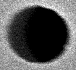
\includegraphics[scale=1.4]{Figures/original.png}};
  	\end{tikzpicture}
  }
\hfill
\subcaptionbox{Detektierte Umfangslinie (weiße Linie)\label{fig:kante}}
  [.3\linewidth]{
	\begin{tikzpicture}
        	\node (pixelsWithCircle) {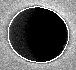
\includegraphics[scale=1.4]{Figures/originalMitKante.png}};
  	\end{tikzpicture}  
  }
\hfill
\subcaptionbox{Einzeichnung eines passenden Kreises mitsamt zugehörigem Radius\label{fig:eingezeichneterKreise}}
  [.3\linewidth]{
	\begin{tikzpicture}
        	\node[anchor=south west] (pixelsWithCircle) at (0,0) {
\includegraphics[scale=1.4]{Figures/edge.png}};
        	\begin{scope}[x={(pixelsWithCircle.south east)},y={(pixelsWithCircle.north west)}]
        	  \coordinate (R1) at (0.5,0.5);
        	  \coordinate (R2) at (0.85,0.5);
          \draw[green, ultra thick,->] (R1) -- (R2) node[midway,above]{$\SI{27}{px}$};
          \draw[green,ultra thick] (R1) ++(0:1.4cm) arc (0:360:1.4cm);
        \end{scope}
  	\end{tikzpicture}  
  }